\documentclass{beamer}
\usepackage[latin1]{inputenc}
\usepackage{tikz}
\usepackage{tikzscale}
\usepackage{pgfplots}

\pgfplotsset{
  /pgfplots/xlabel near ticks/.style={
     /pgfplots/every axis x label/.style={
        at={(ticklabel cs:0.5)},anchor=near ticklabel
     }
  },
  /pgfplots/ylabel near ticks/.style={
     /pgfplots/every axis y label/.style={
        at={(ticklabel cs:0.5)},rotate=90,anchor=near ticklabel}
     }
  }

\usepgfplotslibrary{groupplots}
\usepackage{filecontents}
\usepackage{adjustbox}

\usetheme{Dresden}
\usecolortheme{beaver}
\title[]{Numerical Solutions to Loewner's Equation and Applications}
\author{Dolica Akello-Egwel}
\date{September 4th 2018}

\begin{document}

% Title Page
\begin{frame}
\titlepage
\end{frame}

% Introducing Loewner's Equation
\begin{frame}{Loewner's Equation}
\begin{adjustbox}{max totalsize={.9\textwidth}{.7\textheight},center}
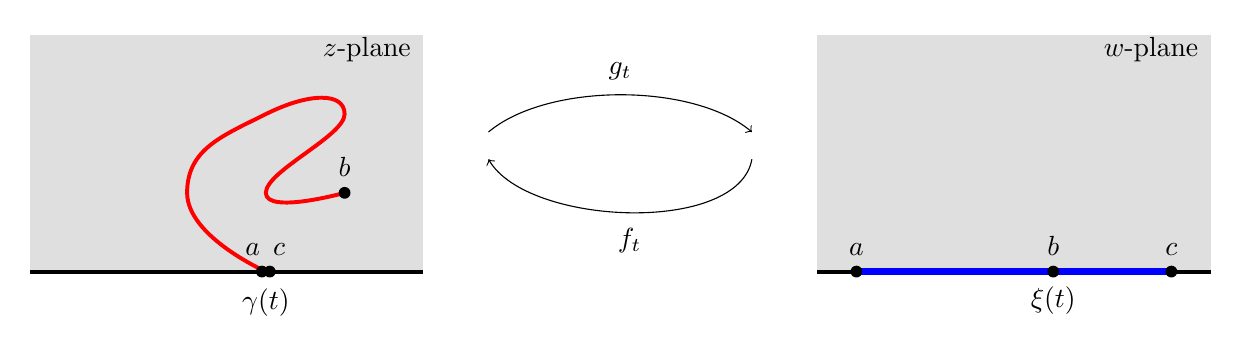
\begin{tikzpicture}
\fill [gray!25] (-3,0) rectangle (2,3);
    \draw [line width=0.5mm,red] plot [smooth, tension=1] coordinates {(0,0) (-1,1) (0,2) (1,2) (0,1) (1,1)};
    \draw [line width=0.5mm, black]  (-3,0) -- (2,0);
    \draw (2,3) node[below=0.5em,left=1pt] {$z$-plane};
    \draw (0,0) node[below=1mm] {$\gamma(t)$};
    \draw (0,0) node[xshift=-0.05cm,circle,black,inner sep=0pt,minimum size=1.5mm,fill,label=$a \ \ $]{};
    \draw (0,0) node[xshift=0.05cm,circle,black,inner sep=0pt,minimum size=1.5mm,fill,label=$\ \ c$]{};
    \draw (1,1)  node[circle,inner sep=0pt, minimum size=1.5mm,fill,label=$b$]{};
    \node[anchor=east,xshift=5cm,circle] at (-2,1.6) (Start) {};
    \node[anchor=west,xshift=5cm,circle] at (1,1.6) (End) {};
    \draw [->,out=40,in=140,looseness=0.75] (Start.north) to node[above=2pt]{$g_t$}  (End.north);
    \draw [->,out=260,in=300,looseness=0.75] (End.south) to node[below=2pt]{$f_t$}  (Start.south);
    \fill [gray!25,xshift=10cm] (-3,0) rectangle (2,3);
    \draw [line width=0.5mm, black,xshift=10cm]  (-3,0) -- (2,0);
    \draw [line width=0.8mm, blue,xshift=10cm]  (-2.5,0) -- (1.5,0);
    \draw (-2.5,0) node[circle,black,inner sep=0pt,xshift=10cm,minimum size=1.5mm,fill,label=$a$]{};
    \draw (0,0) node[circle,black,inner sep=0pt,xshift=10cm,minimum size=1.5mm,fill,label=$b$]{};
    \draw (1.5,0)  node[xshift=10cm,circle,inner sep=0pt, minimum size=1.5mm,fill,label=$c$]{};
    \draw (0,0) node[xshift=10cm,below=2] {$\xi(t)$};
    \draw (2,3) node[xshift=10cm,below=0.5em,left=1pt] {$w$-plane};
\end{tikzpicture}

\end{adjustbox}

$$g_t = \frac{2}{g - \xi(t)} \quad\quad\quad g_0(z) = z$$

Applications:
\begin{itemize}
\item Growth of cracks
\item Formation of stream networks
\item Percolation/self-avoiding walks
\end{itemize}
\end{frame}

% Project Objectives
\begin{frame}{Project Objectives}
\end{frame}

% The Forward Problem
\begin{frame}{The Forward Problem}
\end{frame}

% The Forward Problem - Algorithm (2.1 From Report)
\begin{frame}{The Forward Problem: Algorithm}
\end{frame}

% Linear Driving
\begin{frame}{Linear Driving}
\begin{adjustbox}{max totalsize={.9\textwidth}{.7\textheight},center}
\begin{tikzpicture}
    \begin{groupplot}[
            group style={
                horizontal sep = 45pt,
                group name=left plots,
                group size=2 by 1,
                },
            ymin=0,
            ylabel near ticks,
            height=0.4\textwidth,
            width=0.4\textwidth,
            tick align=inside,
            tick pos=left,
            xmajorgrids,
            x grid style={gray!25},
            ymajorgrids,
            y grid style={gray!25},
            ]
        \nextgroupplot[xlabel={$\operatorname{Re}(z)$},ylabel={$\operatorname{Im}(z)$},]
            \addplot table [col sep=space,mark=none,smooth] {Data/SingleTrace/Forward/1-0-25-1000-10.dat};
        \nextgroupplot[xmin=0,xmax=25,ymax=25,xlabel={$t$},ylabel={${\xi(t)}$},]
            \addplot[color=red] table [col sep=space,mark=none,smooth] {Data/SingleTrace/Inverse/1-0-25-1000-10.dat};
    \end{groupplot}
\end{tikzpicture}

\end{adjustbox}
\end{frame}

\end{document}
